\section{曲面第一基本形式}

参考微分几何例题详解和习题汇编·陈维恒.

正则参数曲面\footnote{正则曲面是二维流形的例子,曲面的每一个正则参数表示给出了一个局部坐标系} $S$ 是满足 $\boldsymbol{r}_{u}\times \boldsymbol{r}_{v}\neq0$ 的连续可微映射
\[
\boldsymbol{r}:D\subset E^2\to E^3\qquad (u,v)\mapsto(x(u,v),y(u,v),z(u,v))
\]
$S$ 在每一点处有确定的标架 $\{ \boldsymbol{r}(u,v);\boldsymbol{r}_{u}(u,v),\boldsymbol{r}_{v}(u,v),\boldsymbol{n}(u,v) \}$,其中
\[
\boldsymbol{n}(u,v)=\frac{\boldsymbol{r}_{u}(u,v)\times \boldsymbol{r}_{v}(u,v)}{\lvert \boldsymbol{r}_{u}(u,v)\times \boldsymbol{r}_{v}(u,v) \rvert }
\]
称一个变换 $(\widetilde{u},\widetilde{v})\to(u,v)$ 为正则参数变换,若
\[
\frac{ \partial (u,v) }{ \partial (\widetilde{u},\widetilde{v}) } \neq 0
\]
而且有足够的可微性.
\[
\mathrm{I}=d \boldsymbol{r}(u,v) \cdot d \boldsymbol{r}(u,v)=E(du)^2+2Fdudv+G(dv)^2
\]
其中 $E=\boldsymbol{r}_{u}\cdot \boldsymbol{r}_{u},G=\boldsymbol{r}_{v}\cdot \boldsymbol{r}_{v},F=\boldsymbol{r}_{u}\cdot \boldsymbol{r}_{v}$.

\subsection{直纹面}

直纹面可以表示为
\[
\boldsymbol{r}=\boldsymbol{a}(u)+v \boldsymbol{l}(u)
\]
其中 $\boldsymbol{a}(u)$ 是直纹面的准现,$\boldsymbol{l}(u)$ 是直母线的方向向量.

\subsubsection{可展曲面}

可展曲面是一种特殊的直纹面. 它的切平面沿每一条直母线是不变的. 曲面 $S$ 是可展曲面的充要条件是
\[
(\boldsymbol{a}'(u),\boldsymbol{l}(u),\boldsymbol{l}'(u))=0
\]
\subsection{例题}

\subsubsection{参数化曲面}

\subsubsection{直纹面的参数方程}

\begin{exercise}
例题 3.2 写出单叶双曲面 $\frac{x^2}{a^2}+\frac{y^2}{b^2}-\frac{z^2}{c^2}=1$ 作为直纹面的参数方程.
\end{exercise}
直接强行因式分解即可.

\subsubsection{验证曲面的正则性}

\begin{figure}[H]
\centering
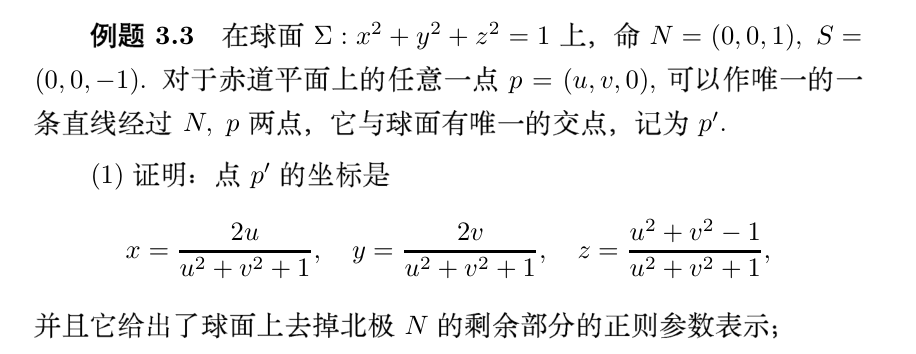
\includegraphics[width=\textwidth]{曲面形式(不严谨)-2025040320.png}
% \caption{}
\label{}
\end{figure}

\subsubsection{验证曲面的可定向性}

\begin{figure}[H]
\centering
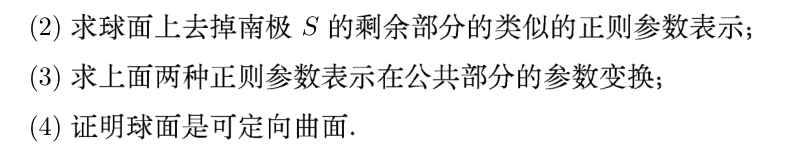
\includegraphics[width=\textwidth]{2-曲面形式(不严谨)-2025040320.png}
% \caption{}
\label{}
\end{figure}

\subsubsection{判断正则参数曲面是球面的一部分}

\begin{exercise}
例题 3.5 证明:一个正则参数曲面是球面的一部分的充分必要条件是,它的所有法线都经过一个固定点.
\end{exercise}
必要性显然,下面考虑充分性:假定曲面 $S$ 的所有法线都经过一个固定点 $\boldsymbol{c}_{0}$, 即存在函数 $\lambda(u,v)$ 使得
\begin{equation}
\boldsymbol{r}(u,v)+\lambda(u,v)\boldsymbol{n}(u,v)=\boldsymbol{c}_{0}
\label{caa238}
\end{equation}

下面证明 $\lambda(u,v)$ 是常值函数. 将 \cref{caa238} 分别对 $u,v$ 求导数得到
\begin{equation}
\boldsymbol{r}_{u}+\lambda \boldsymbol{n}_{u}+\lambda_{u}\boldsymbol{n}=0\qquad \boldsymbol{r}_{v}+\lambda \boldsymbol{n}_{v}+\lambda_{v}\boldsymbol{n}=0
\label{c27a16}
\end{equation}

因为 $\boldsymbol{r}_{u},\boldsymbol{r}_{v}$ 是切向量,又因为单位向量函数 $\boldsymbol{n}$ 的偏导数必定与其它自身正交,因此用 $\boldsymbol{r}$ 与 \cref{c27a16} 做内积得到 $\lambda_{u}=\lambda_{v}=0$. 这说明 $\lambda(u,v)=\lambda_0$,于是
\[
\boldsymbol{r}(u,v)-\boldsymbol{c}_{0}=\lambda_{0}\boldsymbol{n}(u,v)
\]
因此 $\lvert \boldsymbol{r}(u,v)-\boldsymbol{c}_{0} \rvert ^2=\lambda^{2}_{0}$.

\subsubsection{旋转面的充要条件}

\begin{exercise}
例题 3.6 证明:旋转面的法线必定与旋转轴平行或相交;反过来,如果一个正则参数曲面的所有法线都与一条固定的直线相交,则它必定是旋转面.
\end{exercise}
必要性显然. 因为旋转面的参数方程为
\[
\boldsymbol{r}=\boldsymbol{r}(u,v)=(f(u)\cos v,f(u)\sin v,g(u))
\]
其中 $f(u)>0,f'^2(u)+g'(u)>0$.

充分性的证明需要发挥一点几何想象力.不妨假定曲面 $S$ 的所有法线都经过 $z$ -轴,用一个通过 $z$ -轴,并且与 $O x z$ 平面的夹角为 $v$ 的平面截曲面 $S$ ,其截线的参数方程可以假设为 $(u \cos v, u \sin v, g(u, v))$ ,这就是说该截线上的点到 $z$ -轴的距离是 $u$ ,到 $O x y$ 平面的距离是 $g(u, v)$ ,这里 $u$ 是该截线上的参数,$v$ 是任意的固定值.现在要证明:函数 $g(u, v)$ 与 $v$ 无关,因而该曲面 $S$ 就是一个旋转面.\footnote{很明显,当 $v$ 变化时,上面的截线就扫出曲面 $S$ .}

\subsubsection{已知参数方程求第一基本形式}

\begin{exercise}
例题 3.10 设球面的参数方程是(参看例题 3.3(1))
\[
r=\left(\frac{2 u}{u^2+v^2+1}, \frac{2 v}{u^2+v^2+1}, \frac{u^2+v^2-1}{u^2+v^2+1}\right),
\]求它的第一基本形式.
\end{exercise}
直接计算 $E=\boldsymbol{r}_{u}\cdot \boldsymbol{r}_{u},F=\boldsymbol{r}_{u}\cdot \boldsymbol{r}_{v},G=\boldsymbol{r}_{v}\cdot \boldsymbol{r}_{v}$.

\subsubsection{在球面上求与经线成固定角的轨线方程}

\begin{figure}[H]
\centering
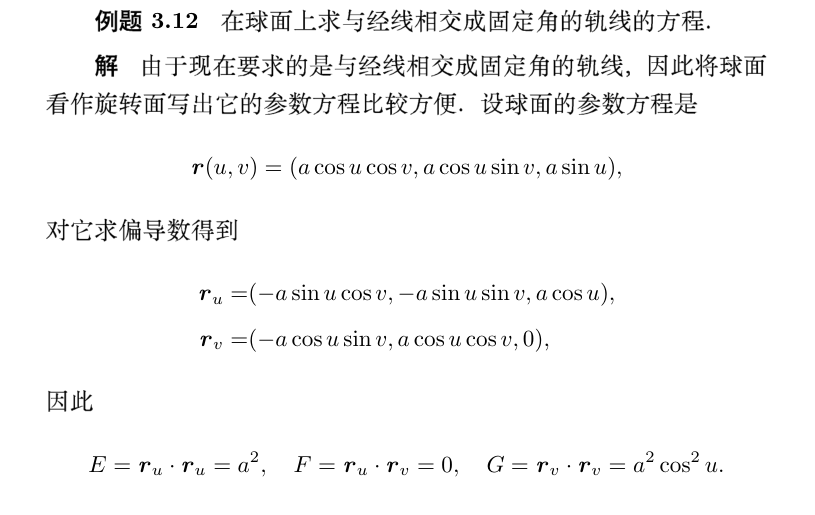
\includegraphics[width=\textwidth]{曲面形式(不严谨)-2025040321.png}
% \caption{}
\label{}
\end{figure}

\begin{figure}[H]
\centering
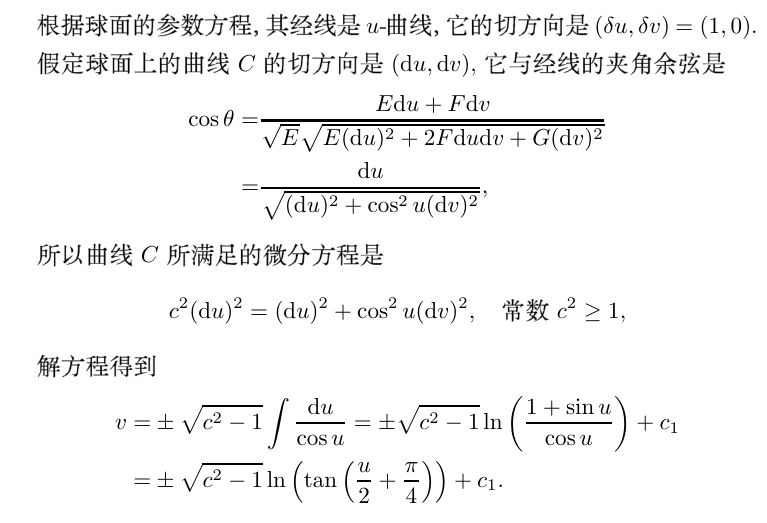
\includegraphics[width=\textwidth]{1-曲面形式(不严谨)-2025040321.png}
% \caption{}
\label{}
\end{figure}

\subsubsection{正交化参数曲面网}

\begin{figure}[H]
\centering
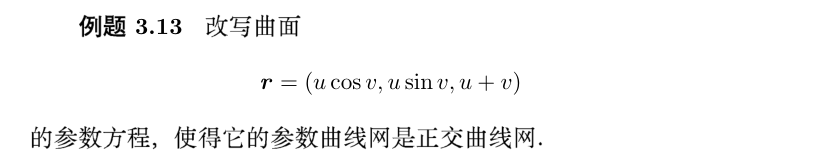
\includegraphics[width=\textwidth]{2-曲面形式(不严谨)-2025040321.png}
% \caption{}
\label{}
\end{figure}

先写成第一基本形式,然后再配方换元.

\subsubsection{求单参数平面族的包络}

\begin{exercise}
求单参数平面族的包络:
\[
x\cos\alpha+y\sin\alpha-z\sin\alpha=1
\]
\end{exercise}
命
\[
F(x, y, z, \alpha)=x \cos \alpha+y \sin \alpha-z \sin \alpha-1
\]
则
\[
F_\alpha(x, y, z, \alpha)=-x \sin \alpha+y \cos \alpha-z \cos \alpha
\]
将方程组 $F=0, F_\alpha=0$ 中的参数 $\alpha$ 消去得到
\[
x^2+(y-z)^2=1
\]
这是一张柱面,属于可展曲面的一种.写成参数方程的形式是
\[
r=(\cos u, \sin u+v, v)=(\cos u, \sin u, 0)+v(0,1,1)
\]
\section{曲面第二基本形式}

曲面第一基本形式描写曲面上与度量有关的性质,曲面第二基本形式描写曲面的形状.

设曲面 $S$ 的参数方程是 $\boldsymbol{r}=\boldsymbol{r}(u,v)$,其单位法向量为 $\boldsymbol{n}(u,v)$,则曲面的第二基本形式为
\[
\mathrm{II}=L(du)^2+2Mdudv+N(dv)^2
\]
其中
\[
\begin{aligned}
L & =\boldsymbol{r}_{u u} \cdot \boldsymbol{n}=-\boldsymbol{r}_u \cdot \boldsymbol{n}_u, \quad N=\boldsymbol{r}_{v v} \cdot \boldsymbol{n}=-\boldsymbol{r}_v \cdot \boldsymbol{n}_v \\
M & =\boldsymbol{r}_{u v} \cdot \boldsymbol{n}=-\boldsymbol{r}_u \cdot \boldsymbol{n}_v=-\boldsymbol{r}_v \cdot \boldsymbol{n}_u
\end{aligned}
\]
在计算系数 $L,M,N$ 时,必须用\textbf{单位法向量}$\boldsymbol{n}=\frac{\boldsymbol{r}_{u}\times \boldsymbol{r}_{v}}{\lvert \boldsymbol{r}_{u}\times \boldsymbol{r}_{v} \rvert}$. \underline{初学者容易犯用} $\boldsymbol{r}_{u}\times \boldsymbol{r}_{v}$ \underline{代替} $\boldsymbol{n}$ \underline{的错误}.

法曲率:
\[
\kappa_n=\frac{L(\mathrm{~d} u)^2+2 M \mathrm{~d} u \mathrm{~d} v+N(\mathrm{~d} v)^2}{E(\mathrm{~d} u)^2+2 F \mathrm{~d} u \mathrm{~d} v+G(\mathrm{~d} v)^2}=\frac{\mathrm{II}}{\mathrm{I}}
\]
正则参数曲面在任意一个固定点,其法曲率必定在两个彼此正交的切方向上分别取最大值和最小值.曲面在一个固定点处沿各个切方向的法曲率的\underline{最大值和最小值}称为曲面在该点的\textbf{主曲率},记为 $\kappa_1, \kappa_2$ ,达到这最大值和最小值的切方向称为曲面在该点的主方向.这个事实可以通过直接计算来证实(参看例题 4.5).若曲面在 $p$ 点的两个彼此正交的主方向单位向量是 $e_1, e_2$ ,对应的\textbf{主曲率}是 $\kappa_1, \kappa_2$ ,则曲面在点 $p$ 沿着与主方向 $e_1$ 的夹角为 $\theta$ 的切方向的法曲率是
\[
\kappa_n(\theta)=\kappa_1 \cos ^2 \theta+\kappa_2 \sin ^2 \theta,
\]
这就是著名的 \textbf{Euler 公式}.

\textbf{Gauss 曲率}


\subsection{求解主曲率和主方向}

\begin{figure}[H]
\centering
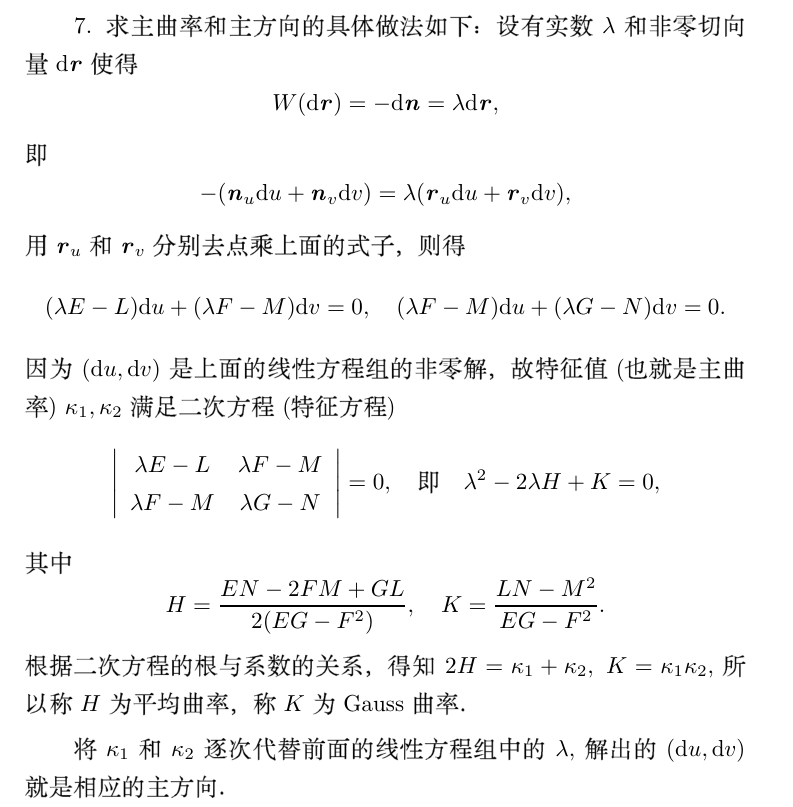
\includegraphics[width=\textwidth]{曲面形式(不严谨)-2025040322.png}
% \caption{}
\label{}
\end{figure}

\subsection{直接求主方向}

\begin{figure}[H]
\centering
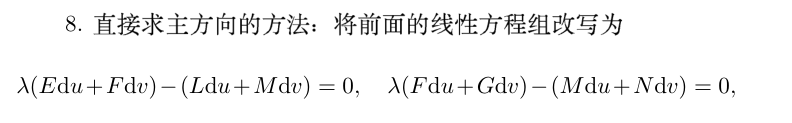
\includegraphics[width=\textwidth]{1-曲面形式(不严谨)-2025040322.png}
% \caption{}
\label{}
\end{figure}

\begin{figure}[H]
\centering
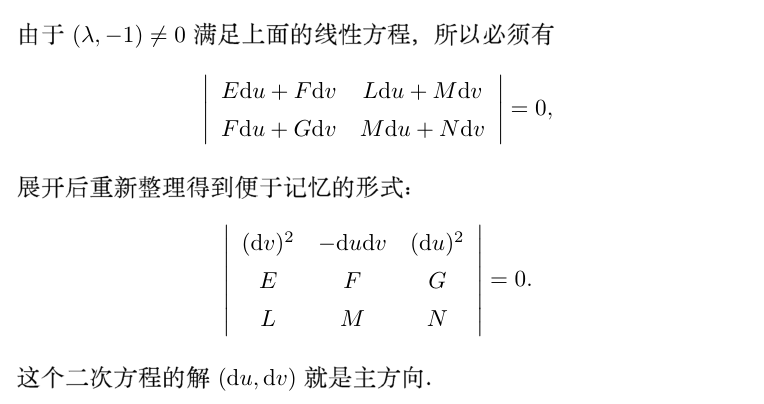
\includegraphics[width=\textwidth]{2-曲面形式(不严谨)-2025040322.png}
% \caption{}
\label{}
\end{figure}

\subsection{渐进曲线}

法曲率为零的切方向称为渐近方向.曲面只在双曲点和抛物点有渐近方向.曲面上其切方向处处是曲面的渐近方向的曲线称为曲面上的渐近曲线.渐近曲线的微分方程是
\[
L(\mathrm{~d} u)^2+2 M \mathrm{~d} u \mathrm{~d} v+N(\mathrm{~d} v)^2=0
\]
\subsection{椭圆点、抛物点、双曲点}

\begin{figure}[H]
\centering
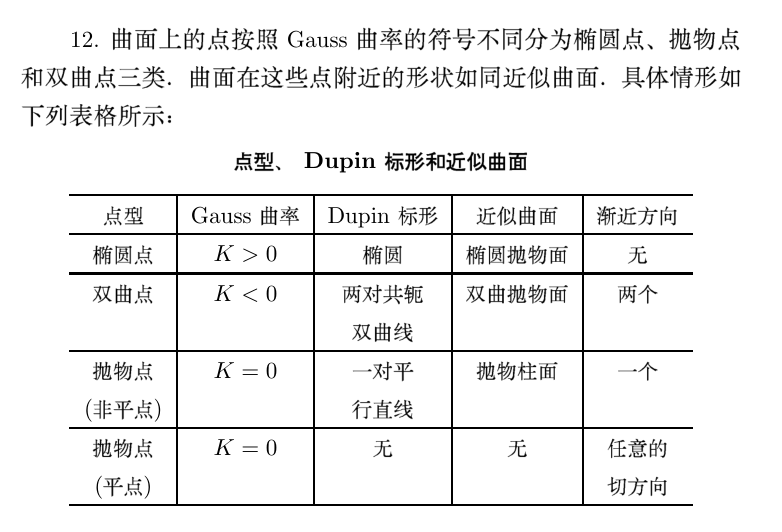
\includegraphics[width=\textwidth]{3-曲面形式(不严谨)-2025040322.png}
% \caption{}
\label{}
\end{figure}

\subsection{例题}

\subsubsection{计算法曲率,主曲率, Gauss 曲率,平均曲率,主方向}

\begin{figure}[H]
\centering
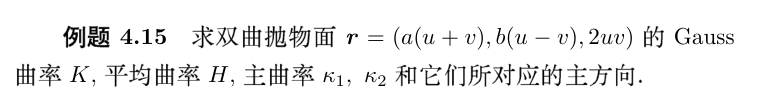
\includegraphics[width=\textwidth]{4-曲面形式(不严谨)-2025040322.png}
% \caption{}
\label{}
\end{figure}

\begin{figure}[H]
\centering
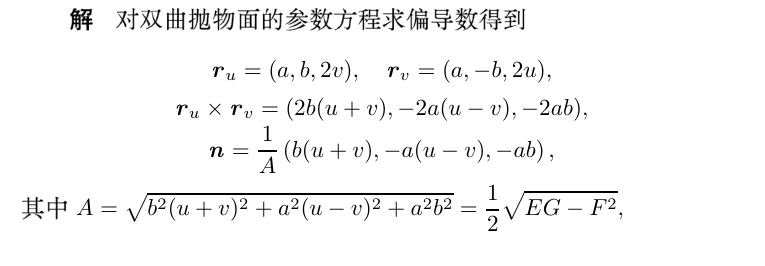
\includegraphics[width=\textwidth]{5-曲面形式(不严谨)-2025040322.png}
% \caption{}
\label{}
\end{figure}
\begin{figure}[H]
\centering
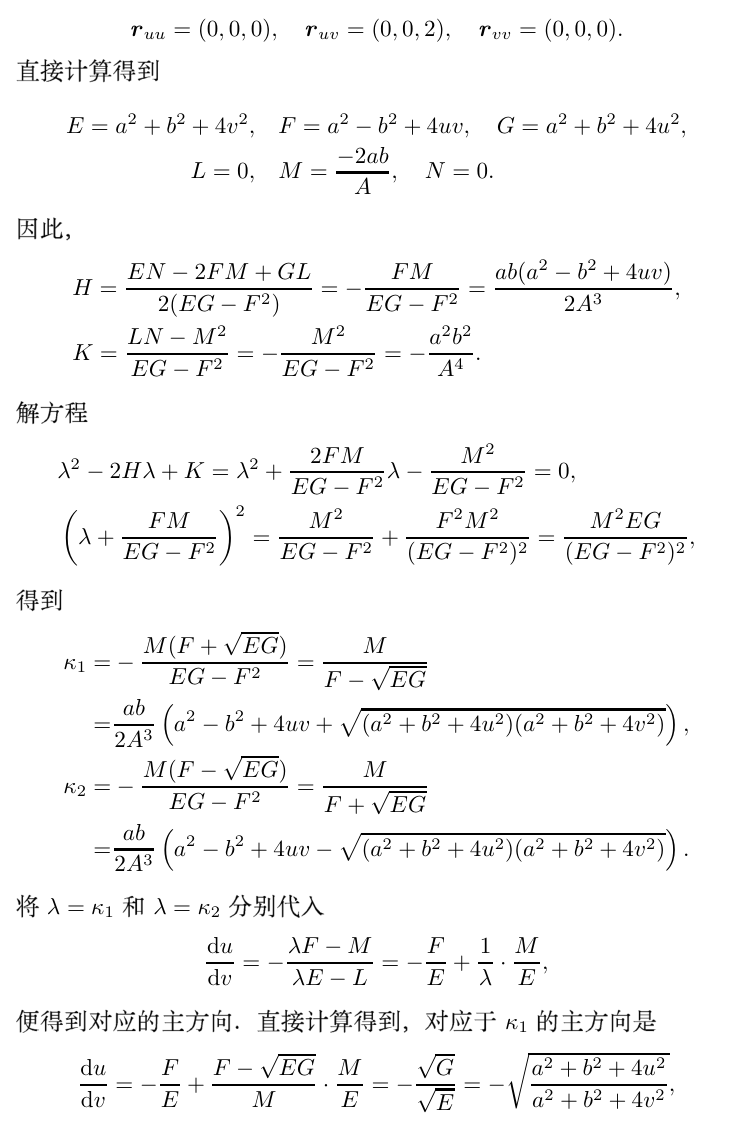
\includegraphics[width=\textwidth]{6-曲面形式(不严谨)-2025040322.png}
% \caption{}
\label{}
\end{figure}
\begin{figure}[H]
\centering
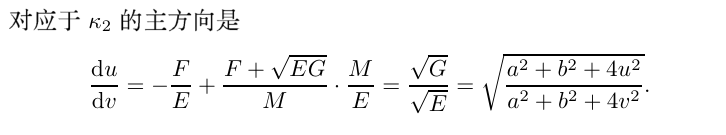
\includegraphics[width=\textwidth]{7-曲面形式(不严谨)-2025040322.png}
% \caption{}
\label{}
\end{figure}
\begin{figure}[H]
\centering
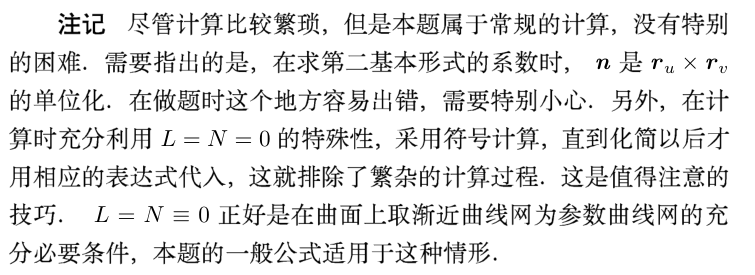
\includegraphics[width=\textwidth]{8-曲面形式(不严谨)-2025040322.png}
% \caption{}
\label{}
\end{figure}

\subsubsection{求脐点}

脐点(Umbilic Point)是微分几何中的一个重要概念,主要用于研究曲面的\textbf{二阶几何性质}(如曲率)。它是指\textbf{曲面的主曲率在该点处相等}的点。

\begin{figure}[H]
\centering
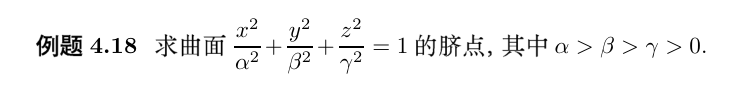
\includegraphics[width=\textwidth]{9-曲面形式(不严谨)-2025040322.png}
% \caption{}
\label{}
\end{figure}
